\documentclass[14pt,a4paper]{scrartcl}
\usepackage[utf8]{inputenc}
\usepackage[english,russian]{babel}
\usepackage{indentfirst}
\usepackage{misccorr}
\usepackage{graphicx}
\usepackage{amsmath}
\usepackage{textcomp}
\usepackage{alltt}
\usepackage{amssymb}
\usepackage{pgfplots}
\graphicspath{{pictures/}}
\begin{document}
\begin{titlepage}
  \begin{center}
    \large
    МИНИСТЕРСТВО ОБРАЗОВАНИЯ И НАУКИ\\ РОССИЙСКОЙ ФЕДЕРАЦИИ
     
    \vspace{0.5cm}
 
    Федеральное государственное автономное образовательное учреждение высшего образования \\ «МОСКОВСКИЙ ФИЗИКО-ТЕХНИЧЕСКИЙ ИНСТИТУТ (научно-исследовательский институт)»
    \vspace{0.25cm}

	Физтех-школа аэрокосмических технологий
     
    Кафедра общей физики
    \vfill
     
     

    Голубятников Сергей
    \vfill
 
    \textsc{Отчёт по лабораторной работе}\\[5mm]
     
    {\LARGE Тепловое излучение}
  \bigskip
     
   3 курс, группа Б03-903
\end{center}
\vfill
 
\newlength{\ML}
\settowidth{\ML}{«\underline{\hspace{0.7cm}}» \underline{\hspace{2cm}}}
\hfill
\begin{minipage}{0.4\textwidth}
  Руководитель работы\\
  \underline{\hspace{\ML}} Л.\,В.~Инжечик\\
  «\underline{\hspace{0.7cm}}» \underline{\hspace{2cm}} 2021 г.
\end{minipage}%
\bigskip
 

\vfill
 
\begin{center}
  Долгопрудный, 2021 г.
\end{center}
\end{titlepage}


\tableofcontents
\addcontentsline{exp}{section}{Заголовок добавить в содержание}
\newpage


\section{Цель работы}

Снять и исследовать спектры излучения различных спектров, характеризовать различные пики в спектрах радиоактивных веществ.


\section{Теория}


	\section{Теоретическое введение}
		В данной работе исследуются сцинтилляционные гамма - спектрометры на основе неорганического кристалла NaI(Tl) и органической сцинтиллирующей пластмассы. При прохождении гамма -квантов через материальную среду образуются электроны , возникающие за счет фотоэффекта,  комптоновского рассеяния и рождения  электрон-позитронных пар.
		\subsection{Фотоэффект}
		Процесс взаимодействия $\gamma$-кванта с электроном, связанным с атомом, при котором электрону передается вся энергия гамма-кванта. При этом электрону сообщается кинетическая энергия $T_e = E_\gamma - I_i$. Фотоэффект существенен для тяжелых атомов, где он идет с высокой вероятностью даже при высоких энергиях гамма-квантов.
		\subsection{Эффект Комптона}
		Упругое рассеяние фотона на свободном электроне, сопровождающееся изменением длины волны фотона. Максимальная энергия образующихся комптоновских электронов соответствует рассеянию на 180\degres и равна 
		\begin{equation}
		    E_{max} = \cfrac{\eta\omega}{1+\cfrac{mc^2}{2\eta\omega}}
		\end{equation}
		\subsection{Процесс образования электрон-позитронных пар}
		Образование пары проходит вблизи электрона или ядра. При этом энергия образующегося ядра отдачи оказывается малой, так что энергия образования пары практически совпадает с энергией покоя электрона. Появившийся электрон теряет энергию на ионизацию среды. Таким образом, вся энергия электрона остается в детекторе. Позитрон будет двигаться до тех пор, пока не остановится, а затем аннигилирует с электроном среды, в результате чего появятся два гамма-кванта. Далее есть три варианта развития событий:
		\begin{enumerate}
		    \item оба кванта не вылетают из детектора, и тогда вся энергия первичного гамма-кванта остается в детекторе
		    \item один из родившихся квантов покидает детектор
		    \item оба кванта покидают детектор
		\end{enumerate}
		Таким образом, каждый происходящий процес вносит свой вклад в энергетический спектр излучения.
		
		Энергии пиков максимальных энергий для комптоновского поглощения зависят от энергии пиков полного поглощения как
	\begin{equation}
		E_{max} = \frac{\hbar \omega}{1 + \frac{m_e c^2}{2 \hbar \omega}}
	\end{equation}
	
	Положение пика обратного поглощения вычисляется по формуле
	\begin{equation}
		E = \frac{\hbar \omega}{1 + \frac{2 \hbar \omega}{m_e c^2}}
	\end{equation}
	
	Форма сигнала ФЭУ имеет вид
	\begin{equation}
		U(t) = const \cdot \exp\left(-\frac{t}{RC}\right)\left(1 - \exp\left(-\frac{t}{\tau_0}\right)\right)
	\end{equation}




\section{Экспериментальная установка}


Принципиальная блок-схема гамма-спектрометра, изучаемого в данной работе, показана на рис. 1.


\begin{center}
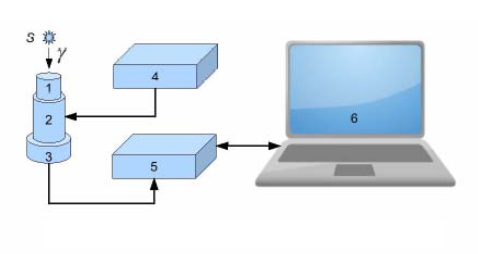
\includegraphics[scale=0.5]{laba.png}\newline
\caption{Рис.1. Схема установки.}
\end{center}

На этом рисунке: 1 - сцинтиллятор, 2 - ФЭУ, 3 - предусилитель импульсов, 4 - высоковольтный блок питания для ФЭУ, 5 - блок преобразования аналоговых импульсов с ФЭУ в цифровой код (АПЦ), 6 - компьютер для сбора данных, их обработки и хранения. 

ФЭУ со сцинтиллятором и блоком питания установлены на отдельной подставке. 




\section{Ход работы}


Проведем измерения гамма-спектров для всех препаратов:\\

\subsection{$^{60} Co$}\\



\begin{center}
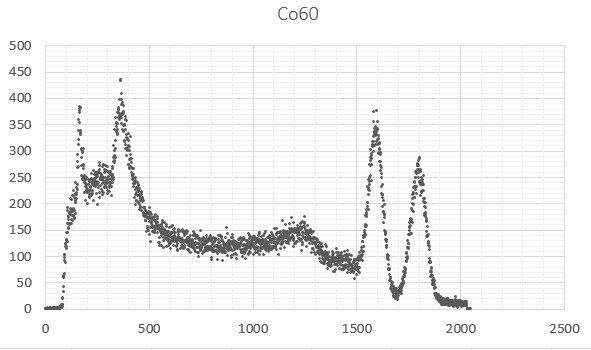
\includegraphics[scale=0.7]{Co.jpg}\newline
\caption{Рис.2. Спектр $^{60} Co$}
\end{center}


\subsection{$^{22} Na$}\\



\begin{center}
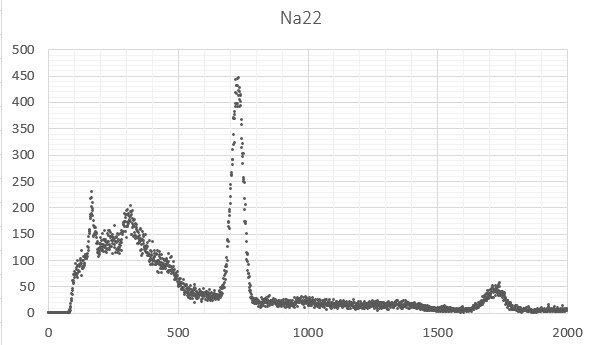
\includegraphics[scale=0.7]{Na.jpg}\newline
\caption{Рис.3. Спектр $^{22} Na$}
\end{center}



\subsection{$^{152} Eu$}\\


\begin{center}
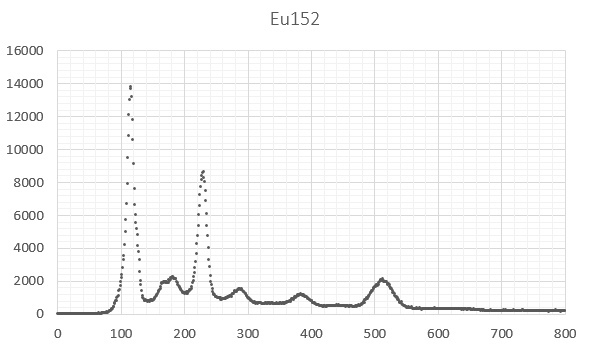
\includegraphics[scale=0.7]{Eu.jpg}\newline
\caption{Рис.4. Спектр $^{152} Eu$}
\end{center}


\subsection{$^{137} Cs$}


\begin{center}
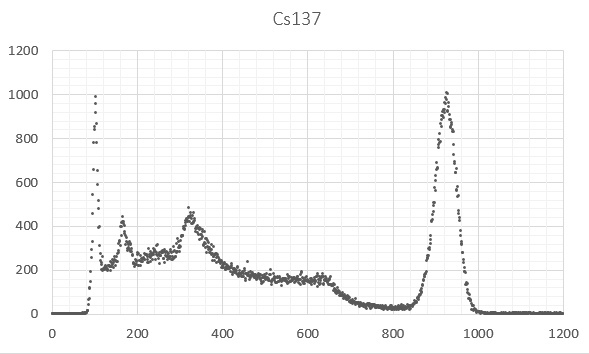
\includegraphics[scale=0.7]{Cs.jpg}\newline
\caption{Рис.5. Спектр $^{137} Cs$}
\end{center}


\subsection{$^{241} Am$}

\begin{center}
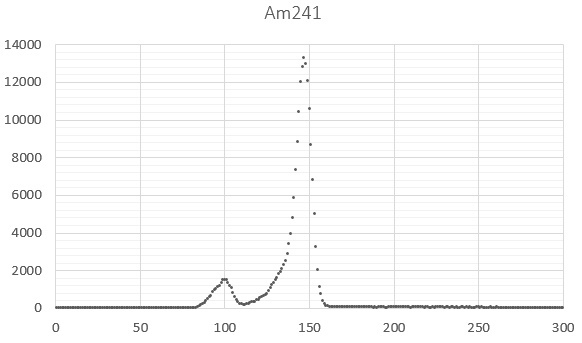
\includegraphics[scale=0.7]{Am.jpg}\newline
\caption{Рис.6. Спектр $^{241} Am$}
\end{center}



Используя известные значения пиков в спектрах натрия и цезия, построим калибровочный график соответствия номера канала определённому значению энергии и получим уравнение для перехода от номера канала к значению энергии в кэВ:


\begin{center}
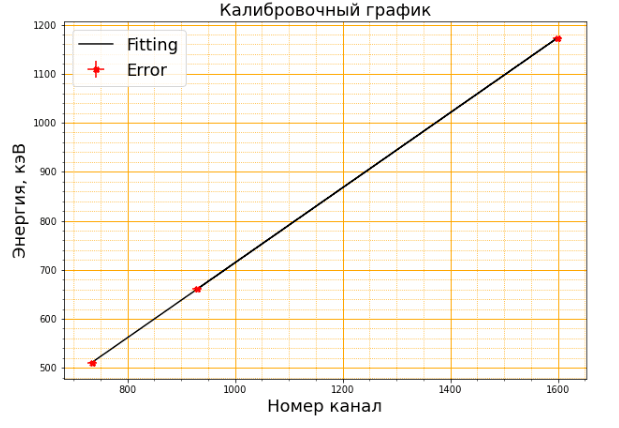
\includegraphics[scale=0.7]{calibr.png}\newline
\caption{Рис.6. Спектр $^{241} Am$}
\end{center}





\begin{center}
    $E = 0.75N_i - 55,2$
\end{center}
где $a = 0.75 \pm 0.02, b = 55.2 \pm 9.0$. Погрешности посчитаны согласно методу наименьших квадратов.\\

Используя калибровочный график, определим значения энергии пиков полного поглощения $E_i$ , их ширины на половине высоты $\triangle E_i$ и энергетическое разрешение $R_i$ . Результаты занесём в таблицу 1. 




\begin{table}[h]
    \centering
    \begin{tabular}{|c|c|c|c|c|c|}
    \hline
        Источник & $N_i$ & $\Delta N_i$ & $E_i$, МэВ & $\Delta E_i$, Мэв & $R_i$\\ \hline
        $^{22} Na$ & 1730 & 123 & 1275 & 94 &  0,074 \\ \hline
        $^{60} Co$  & 1827 & 89 & 1173 & 80 & 0,068\\ \hline
        $^{137} Cs$  & 937 & 75 & 661 & 56 & 0,084\\ \hline
        $^{241} Am$ & 160 & 19 & 67 & 14,8 & 0,220\\ \hline
        $^{152} Eu$  & 526 & 47 & 347 & 36 & 0,104\\ \hline
    \end{tabular}
    \caption{Пики полного поглощения}
\end{table}




Таблица погрешностей:


\begin{table}[h]
    \centering
    \begin{tabular}{|c|c|c|c|c|c|}
    \hline
        Источник & $\sigma_E$ & $\sigma_{\Delta_E}$ & $\sigma_{\Delta_R}$ \\ \hline
        $^{22} Na$ & 34,60 & 1,88 & 0,05  \\ \hline
        $^{60} Co$  & 36,54 & 1,60 & 0,04\\ \hline
        $^{137} Cs$  & 18,74 & 1,12 & 0,06\\ \hline
        $^{241} Am$ & 3,20 & 0,296 & 0,09 \\ \hline
        $^{152} Eu$  & 10,52 & 0,72 & 0,07 \\ \hline
    \end{tabular}
    \caption{Таблица погрешностей}
\end{table}



Построим график зависимости $R^2 = f(1/E)$ на рис.7. Наблюдаем линейную зависимость.

\begin{center}
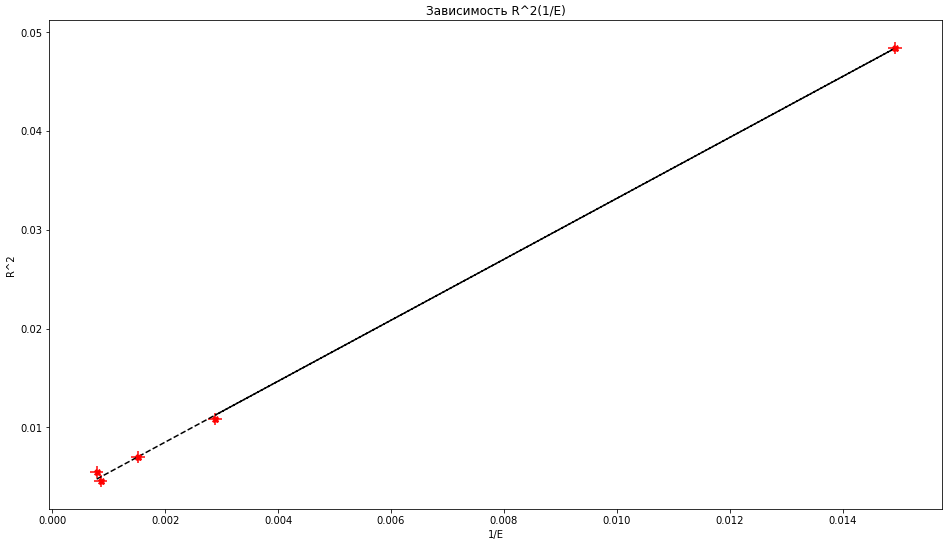
\includegraphics[scale=0.6]{grrrrr.png}\newline
\caption{Рис.7. График зависимости $R^2$ от $1/E$}
\end{center}

Определим энергии края комптоновского поглощения для образцов $^{22}$Na, $^{137}$Cs, $^{60}$Co, сравним их с соответствующими справочными значениями.
\begin{center}
$^{22}$Na: \hspace{1cm} $E_C_{exp} =0,999$ MeV \hspace{1cm} $E_C_{th} = 1.062$ MeV \\
  $^{60}$Co: \hspace{1cm} $E_C_{exp} = 0,922$ MeV \hspace{1cm} $E_C_{th} = 0.963$ MeV \\ 
$^{137}$Cs: \hspace{1cm} $E_C_{exp} =0,448$ MeV \hspace{1cm} $E_C_{th} = 0.477$ MeV \\

 \end{center}



\section{Вывод}



В ходе лабораторной работы был разобран принцип устройства сцинтиллятора. Также был изучен ряд радиоактивных источников и снят спектр образцов $^{22} Na$, $^{137} Cs$, $^{60} Co$, $^{152} Eu$, $^{214} Am$. Был построен график и была проверена линейная зависимость квадрата спектрального разрешения прибора от величины, обратной энергии полного поглощения.    
	






\addcontentsline{toc}{section}{Список используемой литературы}

\newpage

\begin{thebibliography}{}

\bibitem{Sulsky1994}
Лабораторный практикум по общей физике: Учеб. пособие для вузов. Т. 3. Квантовая физика / Игошин Ф.Ф., Самарский Ю.А., Ципенюк Ю.М.; Под ред. Ципенюка Ю.М. - М.:Физматкнига, 2005. 432 стр.



	
\end{thebibliography}

\end{document}
